% biber
\documentclass[conference]{IEEEtran}


\usepackage[pdftex]{graphicx}
\graphicspath{{../pdf/}{../jpeg/}}

\usepackage{amsmath}
\usepackage{hyperref}
\hypersetup{
    colorlinks=true,
    linkcolor=blue,
    filecolor=magenta,      
    urlcolor=cyan,
}
\usepackage{placeins}
\usepackage[backend=biber]{biblatex}
\addbibresource{references.bib}

% correct bad hyphenation here
\hyphenation{op-tical net-works semi-conduc-tor}
\makeatletter
\patchcmd{\@verbatim}
  {\verbatim@font}
  {\verbatim@font\small}
  {}{}
\makeatother

\begin{document}
\title{Using Scapy for \\ Man-in-the-Middle Attacks}

\author{
    \IEEEauthorblockN{Ana Rita Martinho}
    \IEEEauthorblockA{Department of Electrical and Computer Engineering\\
        Faculty of Engineering of University of Porto\\
        up201709727@fe.up.pt}
    \and
    \IEEEauthorblockN{Gonçalo Xavier}
    \IEEEauthorblockA{Department of Electrical and Computer Engineering\\
        Faculty of Engineering of University of Porto\\
        up201604506@fe.up.pt}
}

\maketitle

\begin{abstract}
    A Man-in-the-Middle(MITM) attack is a type of cyberattack where an attacker
    secretly relays and possibility alters the communication between 2 
    unsuspecting parties.
    Most recent cryptographic protocols include some form of endpoint 
    authentication specifically to prevent MITM attacks. 
    
    The goal of this project is to demonstrate, using scapy, why such 
    measurements are needed.
    Scapy is a python module that enables a user to send, sniff and forge 
    network packets, as such it provides easy methods to the types of 
    functionalities needed to run a MITM attack.
    
    4 different protocols were analyzed (FTP, SNMP, Telnet and SMTP).

\end{abstract}

\section{Introduction}

This paper will focus on the work developed for the main project of the 
Security for Systems and Networks course.

% !TeX root = ssre.tex
\section{Used tools - Related concepts}

\subsubsection{Scapy}

~\newline
Scapy is a powerful python interactive packet manipulation program. 
It is able to forge or decode packets of a wide number of protocols, send them on the wire, capture them, match requests and replies, and much more. 
Scapy can easily handle most classical tasks like scanning, tracerouting, probing, unit tests, attacks or network discovery. 
It can replace hping, arpspoof, arp-sk, arping, p0f and even some parts of Nmap,
tcpdump, and tshark.

Scapy also performs a lot of other specific tasks that most other tools can’t 
handle, like sending invalid frames, injecting your own 802.11 frames, 
combining techniques (VLAN hopping+ARP cache poisoning, VOIP decoding on WEP 
encrypted channel, …), etc.
As such, it allows its users to easily craft the exact packets they would like,
send them out into the network and analyse their responses.

In the context of this project, the Scapy module was used as the primary tool 
of the developed code, specially its custom packet building functionalities.


\begin{figure}[h!]
    \centering
    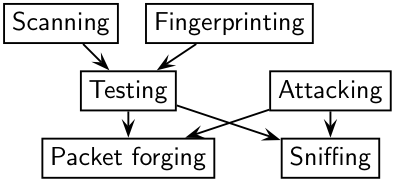
\includegraphics[width=1\linewidth,keepaspectratio]{taxonomy.png}
    \caption{Scapy's taxonomy as depicted in \cite{scapy}}
    \label{fig:taxonomy}
\end{figure}
\FloatBarrier

~
\subsubsection{ARP spoofing}

~\newline
As mentioned in the section \ref{sec:Intro}, the general MITM attack goes 
through 3 main steps: Evesdropping, Positioning and Exploiting. 
\textit{ARP spoofing} played a major role in this project's first and middle 
step.

The ARP protocol is normally used to resolve the specific MAC address associated
with a particular IP, so that packets can reach the intended device - 
translating Layer-3 addresses into Layer-2.
On normal circumstances, the sending device sends an ARP Request to discover the
MAC address of a particular IP.
This request is then broadcasted to the network and the device with the 
specified IP sends an ARP Response announcing its MAC address.

This process can be bypassed by sending an unsolicited ARP Response to a 
specific user, announcing that a particular IP actually belongs to the 
attacker's MAC address.
In the most common form of \textit{ARP spoofing}, the attacker forges an ARP 
Response packet declaring that its MAC address is the one associated with the
active Access Point (AP) IP. 
The attacker then informs the actual AP (in a similar way) that its MAC address
is the one associated with the victims IP.
This way the attacker inserts itself in the middle of all communications 
between the victim and the network, and is able to analyse all the victim's 
traffic.

~
\subsubsection{TCP hijack}

~\newline
An alternative method to accomplish the \textbf{Positioning} step of section
\ref{sec:Intro} is \textit{TCP hijacking}. 

During TCP's three-hand handshake, the client initially sends a random value to
be used as its sequence number (Seq.A), and the server replies with an 
acknowledgment number (ACK) of Seq.A + 1 and a random value value of its own, 
sequence number (Seq.B).
This values are then used to re-arrange out of order packets and ensure that 
the correct packet is received during communication.

An attacker can impersonate one of the involved parties by forging an IP packet 
with the correct ongoing Seq. and ACK values. 
If that happens, the victim's own Seq. and ACK numbers became offsetted, and 
their packets are dropped when reaching the other side of the conversation.
As such, the attacker is able to "hijack" the ongoing connection.

This approach faces some problems: 
\begin{itemize}
    \item \underline{It requires a ongoing connection} - upon receiving a forged
        SYN packet, the server will reply with a SYN ACK to the IP of said 
        packet. 
        Since the real device of this IP did not start a connection, it will
        respond with a TCP packet whose RST bit is set, immediately closing the
        connection.

    \item \underline{The server, and client became aware of the 
        hijack} - it's possible that the large quantity of sudden dropped 
        packets trigger some kind of security alert and this may cause the 
        connection to be dropped.
\end{itemize}

Both these problems can be somewhat dealt with by conditioning not only 
when this attack may occur, but also by closing the real client's connection 
before the hijack, without the server realizing it.

~
\subsubsection{RST attack}

~\newline
Each TCP packet has a header, and each header contains a bit known as the 
"reset" (RST) flag. 
In usual TCP traffic, this bit is set to 0 and has no effect.
However, if this bit is set to 1, it indicates to the receiving device that 
it should immediately stop using the TCP connection; 
it should not send any more packets using the connection's identifying numbers, 
called ports, and discard any further packets it receives with headers 
indicating they belong to this connection. 
A TCP reset basically kills a TCP connection instantly. 

As seen previously, it's possible to inject a forged TCP packet into a ongoing 
TCP connection, if the forged Seq. and ACK numbers are correct. 
As such, an attacker can prematurely terminate a TCP connection, without the 
willing consent of the parties involved.

~
\subsubsection{Reverse Shell}

~\newline
In a typical remote access scenario, the user is the client and the target 
machine is the server. 
The user initiates a remote shell connection and the target system listens 
for such connections. 
With a reverse shell, the roles are the opposite. 
The target machine initiates the connection to the user, and the 
user’s device listens for incoming connections on a specified port.
This can be used to bypass firewall restrictions on open ports, as most 
restrictions are imposed on incoming traffic, not on outgoing one.
Reverse shells can usually be used after some initial code or packet is 
injected in the target machine and allow an attacker to obtain a interactive 
shell session on the victim's machine.


\section{Solution}

Here you should describe the solution.

% !TeX root = ssre.tex
\section{Results}
Before any type of attack, the attacker is prompted by the program with the choice of the victims' IP - based on the ARP table - and the type of attack desired, based on FTP, SNMP, Telnet or SMTP . This workflow is shown in figure \ref{fig:WorkFlow}.

\begin{figure}[h!]
    \centering
    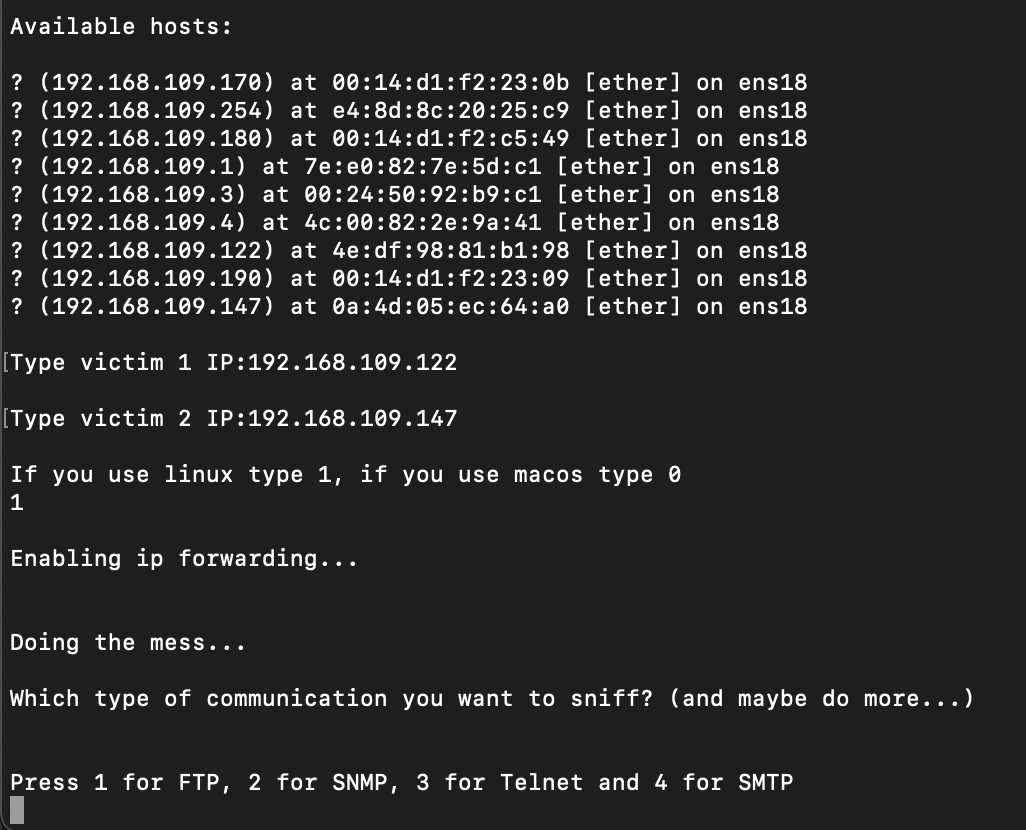
\includegraphics[width=0.85\linewidth,keepaspectratio]{Choice.png}
    \caption{Choice of victims and desired attack}
    \label{fig:WorkFlow}
\end{figure}
\FloatBarrier

The demonstration of the FTP passive attack was accomplished by creating a user and password associated to a FTP account that the FTP server recognizes as being valid. As depict in figure \ref{fig:FTPAttack}, one of the victims (\textit{192.168.109.122}) is accessing the FTP server located at \textit{192.168.109.147} and the attacker (left in the figure) has real-time access to the user and pass as valid credentials. 

\begin{figure}[h!]
    \centering
    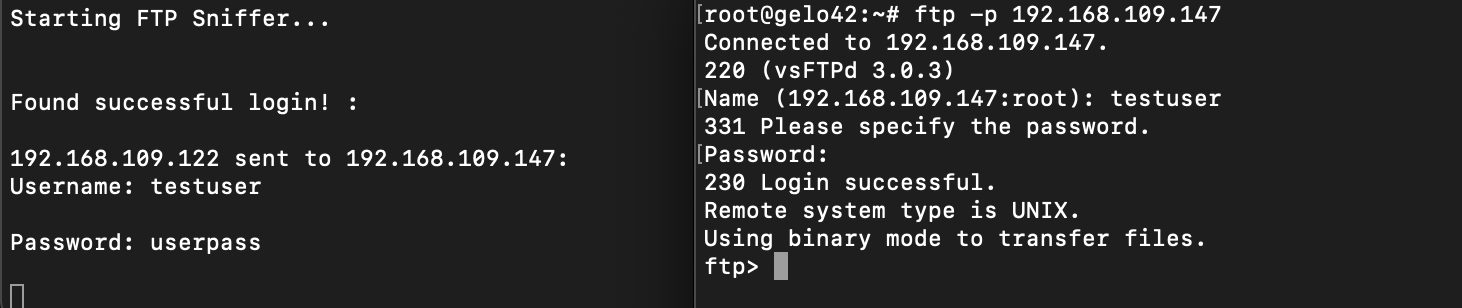
\includegraphics[width=1\linewidth,keepaspectratio]{FTPAttack.png}
    \caption{FTP passive attack}
    \label{fig:FTPAttack}
\end{figure}
\FloatBarrier

For the demonstration of both SNMP active and passive attack, the below described environment was created: 
\\\\
As shown in figure \ref{fig:SNMPPassiveAttack}, a remote user is querying the machine at \textit{192.168.109.147} about its System Up Time, using a \textit{snmpget} command. The attacker (left in the figure) is prompted with real-time data about the response to that command, including the community string \textit{veryprivate}. To perform the active attack, the user must type \textit{Ctrl-C} and enter, as described in section \ref{sec:Solution}, the necessary information. As depicted in figure \ref{fig:SNMPActiveAttack}, the victim of this attack in this created environment is running Debian with kernel version 4.19, it's a 64bit OS and the hostname is "gelo43". Those types of information can be useful for any other type of attacks. 

\begin{figure}[h!]
    \centering
    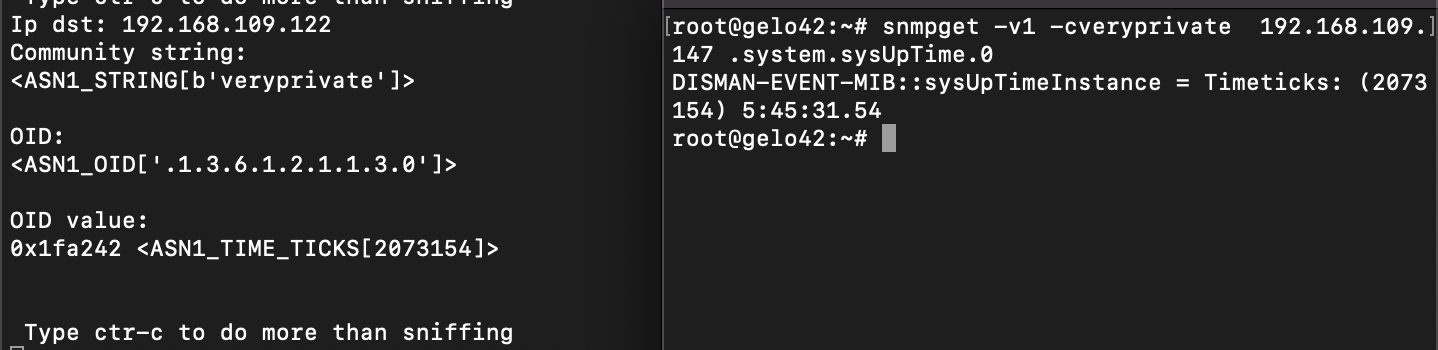
\includegraphics[width=1\linewidth,keepaspectratio]{SNMPSniffing.png}
    \caption{SNMP passive attack}
    \label{fig:SNMPPassiveAttack}
\end{figure}
\FloatBarrier

\begin{figure}[h!]
    \centering
    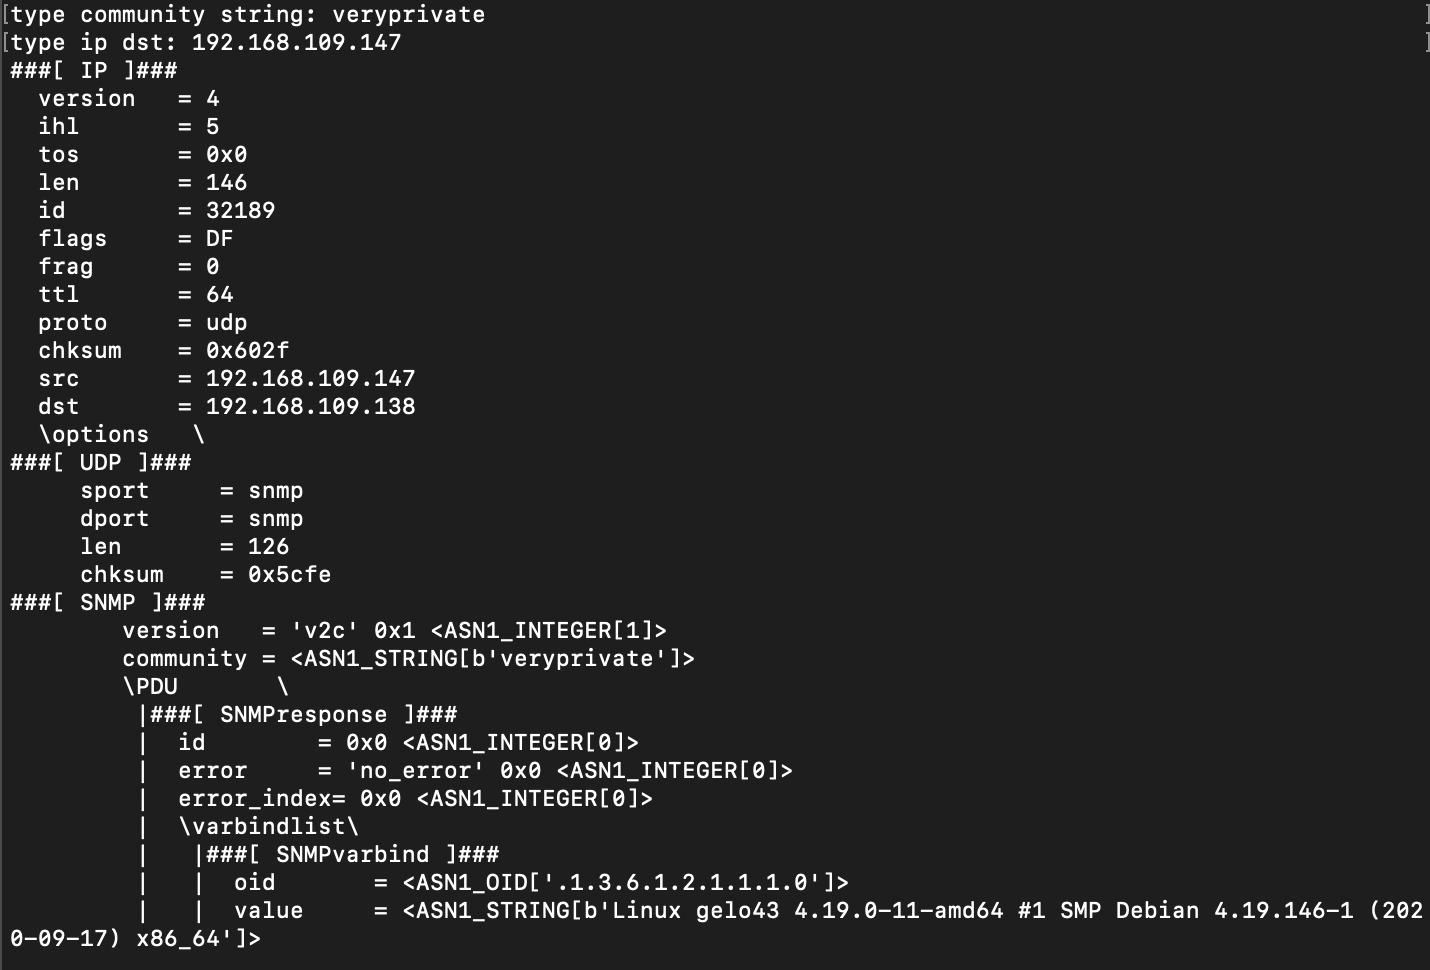
\includegraphics[width=1\linewidth,keepaspectratio]{SNMPAttack.png}
    \caption{SNMP active attack}
    \label{fig:SNMPActiveAttack}
\end{figure}
\FloatBarrier

In order to demonstrate both the passive and active Telnet attacks, the setup
present in \ref{fig:TelnetAttack} was implemented.
One VM was used as a legitimate client for the Telnet service while the 
attacker simultaneously intercepted and sniffed its connection - allowing the 
attacker to passively collect all the client's traffic.
After both victims were identified (Telnet's client and server), the attacker 
launches the mentioned reverse shell and waits for it on a running netcat 
instance - which can be seen in the right part of figure \ref{fig:TelnetAttack}.
Finally, the user's legitimate connection is shutdown due to the aforementioned 
RST forged packet sent by the attacker to the server.

\begin{figure}[h!]
    \centering
    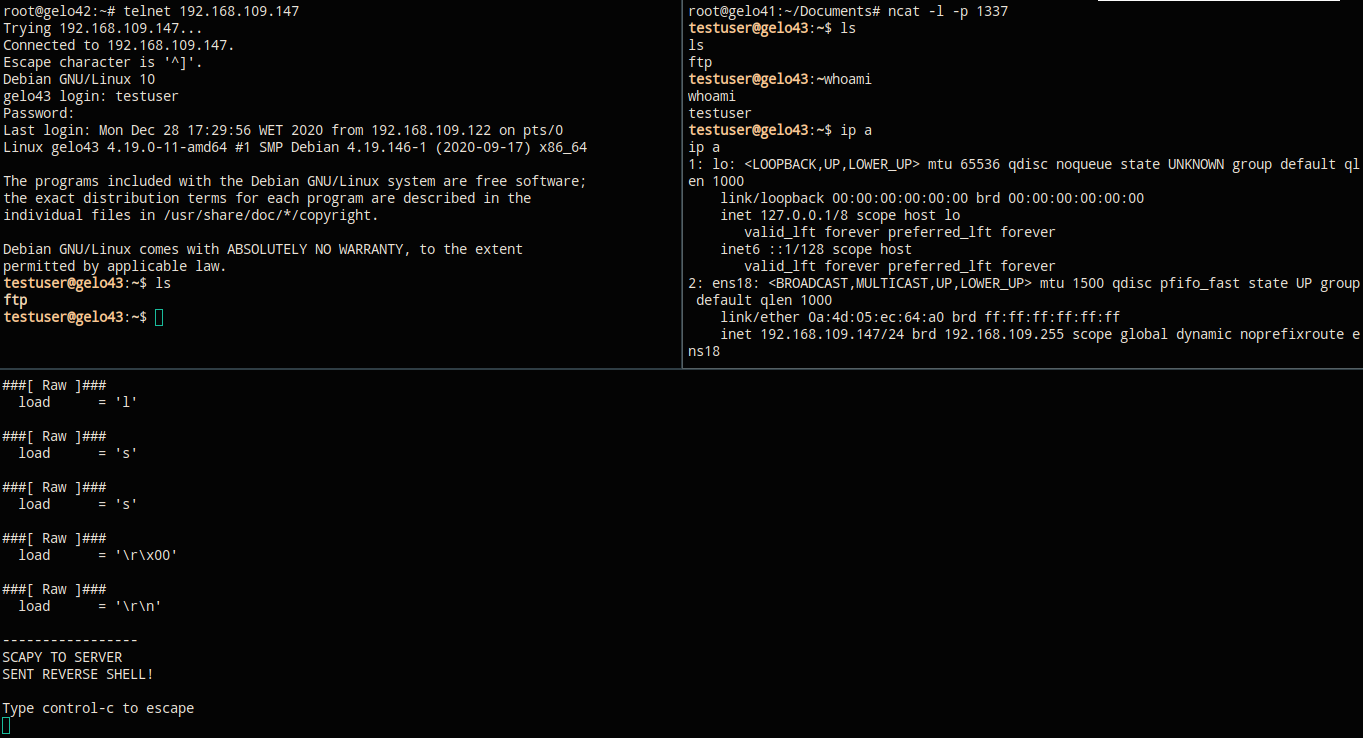
\includegraphics[width=1\linewidth,keepaspectratio]{ReverseShell.png}
    \caption{Telnet active attack - user in top-left, attacker reverse shell 
            in top-right, attacker Scapy bottom}
    \label{fig:TelnetAttack}
\end{figure}
\FloatBarrier


For the demonstration of the SMTP passive attack, one of the victims is \textit{telnetting} to the SMTP Postfix server located at \textit{192.168.109.147}. The victim sends a regular email to the server and, as shown left in figure \ref{fig:SMTPPassiveAttack}, the attacker has access to the user sending email, the receiver and the email body. 
\begin{figure}[h!]
    \centering
    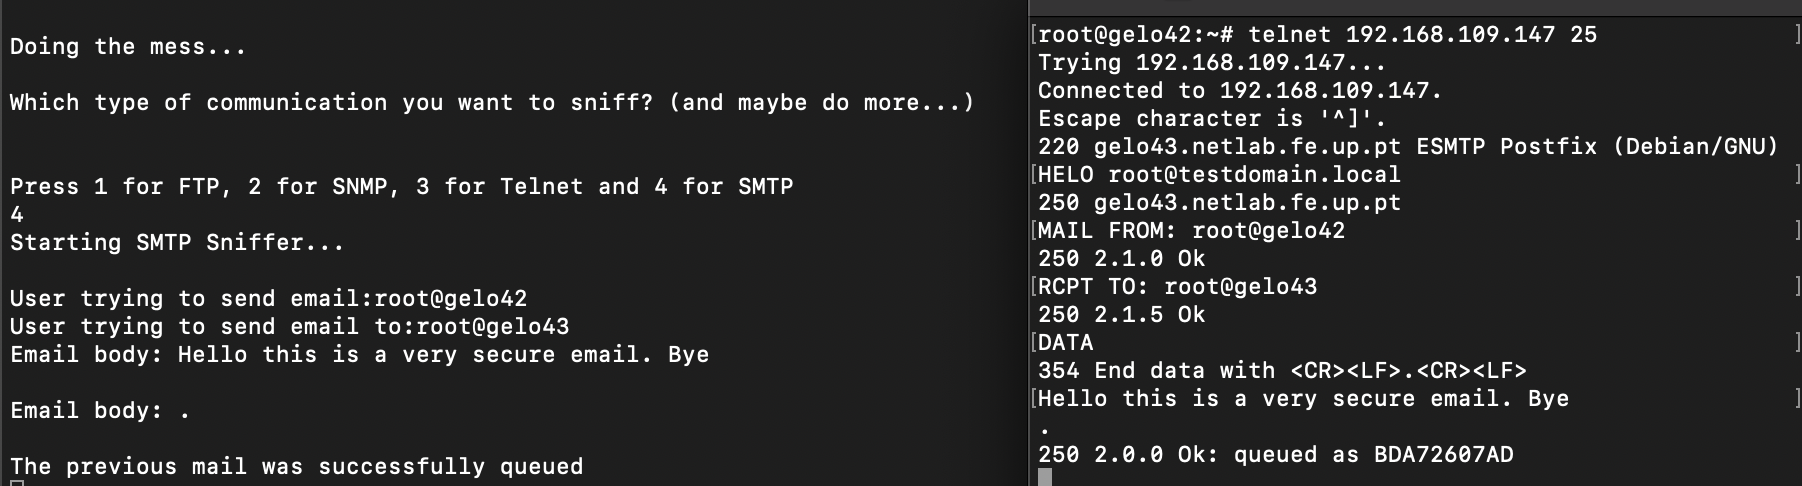
\includegraphics[width=1\linewidth,keepaspectratio]{SMTPAttack.png}
    \caption{SMTP passive attack}
    \label{fig:SMTPPassiveAttack}
\end{figure}
\FloatBarrier

Finally, the entire of the developed project can be found on our own personal
repositories at \url{https://github.com/RitaMartinho/SSRE}.

% !TeX root = ssre.tex
\section{Conclusion}
\label{sec:Concl}

Through this project we were able to have a 1st hand experience with the 
procedures involved in a MITM attack, the security flaws present in the types
of services that fall victim to them and their glaring consequences.

In a general fashion, most of the compromised services analysed would have been 
safe if their communications were implemented on top of 
\underline{encrypted channels} - rendering the attackers interpretation of the 
detected information useless.
In fact, encryption also plays an extremely important role against the
\textbf{Evesdropping} step mentioned in section \ref{sec:Intro}, since no 
identifying content can be detected by the attacker if all traffic is encrypted.

Prevention of the \textbf{Positioning} attacker's step can be done by not 
accepting any unsolicited ARP responses or by some sort of cross-checking of 
ARP responses involving the DHCP server such that both dynamic and static IP
addresses are verified.

In summary, this project showed us how important concepts like encryption 
really are in a practical way.
A special high note should be given to Scapy, not only for its ease of features 
(and implementation), but also its documentation and available resources.


\nocite{*}
\printbibliography

% that's all folks
\end{document}
